\section{Ejercicio 5}

Implementado el Scheduler Round-Robin, se desea analizar ciertos parámetros de calidad del scheduler comparando los mismos para un quantum de 2, 10 y 50 ciclos.
El lote de tareas para la prueba consiste en el siguiente:

\begin{verbatim}
*3 TaskCPU 50 
*2 TaskConsola 5 3 3
\end{verbatim}

Que especifica tres tareas con uso de CPU durante 50 ciclos y 2 tareas que realizan 5 llamadas bloqueantes con duracion de 3 ciclos cada una.\\

Los parámetros de calidad a analizar son: latencia, waiting time y tiempo total de ejecución, siendo la latencia el tiempo que la tarea pasa en estado ''listo'' hasta que comienza su ejecución, el waiting time el tiempo que pasa una tarea sin ejecutar desde el momento que está en estado ''listo'' hasta que termina su ejecución, y el tiempo total de ejecución el tiempo que toma la tarea desde que está en estado ''listo'' hasta que cumple con su ejecución.

\begin{figure}[h]
  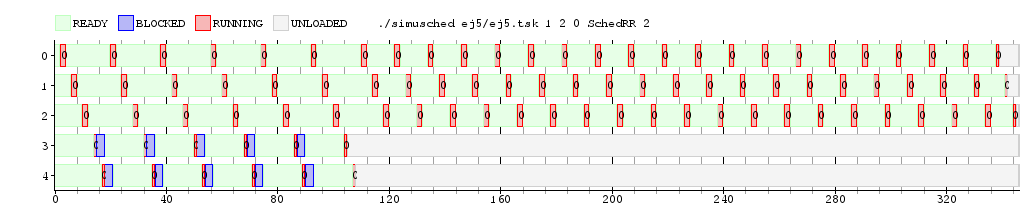
\includegraphics[width=\textwidth]{../ej5/ej5RR1202.png}
  \caption{Tareas con quantum 2.}
  \label{fig:quant2}
\end{figure}


\begin{figure}[h]
  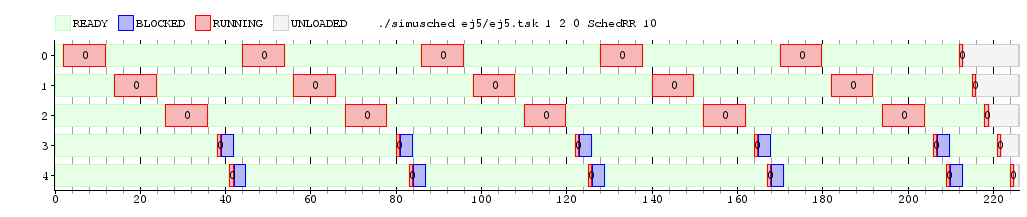
\includegraphics[width=\textwidth]{../ej5/ej5RR12010.png}
  \caption{Tareas con quantum 10.}
\end{figure}


\begin{figure}[h]
  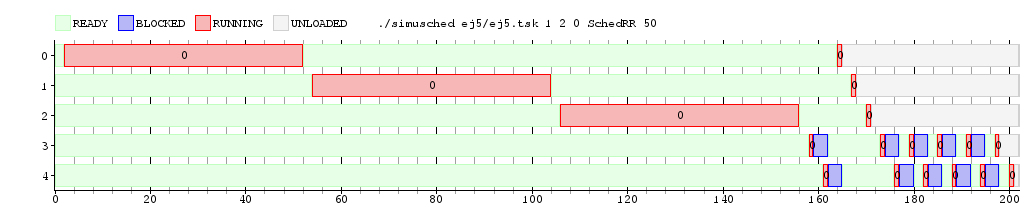
\includegraphics[width=\textwidth]{../ej5/ej5RR12050.png}
  \caption{Tareas con quantum 50.}
\end{figure}















 \begin{table}[h!]
 	\begin{center}
 		\caption{Parámetros de calidad para el sceduler round robin: SchedRR.}
 		\label{tab:table1}
 		\begin{tabular}{|l|c|c|c|c|c|}
 			\hline
 			& Tarea & Latencia & Waiting time & Total ejecución & Ratio (Espera/total) \\
 			\hline
 			\hline
 			& 0 & 2 & 288 & 339 & 0.85\\ \cline{2-6}
 			& 1 & 6 & 291 & 342 & 0.85 \\ \cline{2-6}
 			Quantum = 2 & 2 & 10 & 294 & 345 & 0.85 \\ \cline{2-6}
 			& 3 & 14 & 99 & 105 & 0.94 \\ \cline{2-6}
 			& 4 & 17 & 102 & 108 & 0.94 \\ \cline{2-6}
 			& Avg & 9.8 & 214.8 & 227.8 & 0.89 \\
 			\hline
 			\hline
 			& 0 & 2 & 162 & 213 & 0.76 \\ \cline{2-6}
 			& 1 & 14 & 165 & 216 & 0.76 \\ \cline{2-6}
 			Quantum = 10 & 2 & 26 & 168 & 219 & 0.76 \\ \cline{2-6}
 			& 3 & 38 & 216 & 222 & 0.97 \\ \cline{2-6}
 			& 4 & 41 & 219 & 225 & 0.97 \\ \cline{2-6}
 			& Avg & 24.2 & 186 & 219 & 0.84 \\
 			\hline
 			\hline
 			& 0 & 2 & 114 & 165 & 0.69 \\ \cline{2-6}
 			& 1 & 54 & 117 & 168 & 0.69 \\ \cline{2-6}
 			Quantum = 50 & 2 & 106 & 120 & 171 & 0.70\\ \cline{2-6}
 			& 3 & 158 & 192 & 198 & 0.97 \\ \cline{2-6}
 			& 4 & 161 & 195 & 201 & 0.97 \\ \cline{2-6}
 			& Avg & 96.2 & 147.6 & 180.6 & 0.80 \\
 			\hline
 		\end{tabular}
 	\end{center}
 \end{table}


\clearpage   %con esto todo se arregla!!!!
